\section{Synthetic map generation}
\label{sec:generation}

In order to instruct the CNN to extract the $\dnds$ from the \fermi photon-count map, we need to produce synthetic analogs of the map, constructed from a wide selection of $\dnds$ and for the same characteristics (detector exposure and PSF, known physical foregrounds) of the data we will be using. These maps will then be partly used to train a CNN and partly used to validate the CNN, to determine its performance and to
estimate the uncertainty on the reconstructed $\dnds$. Finally, we will apply the trained CNN to the \fermi data. 

The gamma-ray maps are modeled as the sum of three contributions:
\begin{itemize}
\item A population of gamma-ray point sources. Since our analysis will be restricted to the high galactic latitude region (in order to minimize in the analysis the impact of the galactic foreground emission, as discussed in the following sections), these sources will mostly be of extra-galactic origin and can therefore be assumed to be distributed homogeneously across the sky. 
The high galactic latitude sky also contains a population of millisecond pulsars which can also be approximately assumed to be isotropically distributed \cite{Fermi-LAT:2013svs}, and thus are ideally included in our phenomenological $\dnds$.
In terms of photon flux, the sources are extracted, for each map realization, from the input $\dnds$ distributions, modeled as in Section \ref{sec:dnds}.

\item Diffuse gamma-ray emission from the Milky Way. Galactic emission is the dominant contribution at low galactic latitudes, with a declining intensity at high latitudes. We model the galactic emission as discussed in Section \ref{sec:galactic}, by adopting a template model normalized to the \fermi data. 
Stability of the results against foreground modeling will be tested through the adoption of different templates.

\item An isotropic background, which integrates all source emissions which are too faint to be processed by the CNN and possible truly diffused emission mechanisms, such as gamma-rays from cosmological cascades from ultra high energy cosmic rays or a possible contribution from dark matter annihilation or decay, as well as a residual instrumental CR background contamination. This term is modeled as a constant.

\end{itemize}
\noindent
%
A flux map ${\cal M}$ will therefore be obtained as the sum of three contributions:
\begin{equation}
    {\cal M} = {\cal S} + A_\textrm{gal} \cdot {\cal G} + \fiso
    \label{eq:map}
\end{equation}
where $\cal S$ is the map due to the underlying distribution of sources (obtained from a $\dnds$ model as described in the next subsection), ${\cal G}$ is a template map for the foreground emission and $\fiso$ is a constant that denotes the isotropic component discussed above. The constant $A_\textrm{gal}$ is a normalization constant for the galactic foreground template. 

The count map {$\cal N$} is then obtained by multiplying the flux map by the \fermi exposure map {$\cal E$}, depicted in Fig. \ref{fig:exposure}, and by taking into account the steradian-to-pixel conversion factor. Specifically, the counts in pixel $a$ are obtained as:
\begin{equation}
    {\cal N}_a = {\cal M}_a \cdot {\cal E}_a \cdot \frac{4\pi}{N_\textrm{pix}}
    \label{eq:count}
\end{equation}
%
where the number of pixels in the Healpix scheme is $N_\textrm{pix} = 12\cdot N^2_\textrm{side}$ with $N_\textrm{side} = 2^{n}$ with $n$ the pixeling order.

Since the exposure slightly changes with energy, the above procedure could be improved by performing a convolution in energy of the photon flux with the exposure, instead of directly multiplying the two quantities as performed in Eq. (\ref{eq:count}). However, the gradient in energy of the exposure in the $(1,10)$ GeV energy range is small, and the two procedures would provide very similar results.  We, thus, use the simpler procedure outlined above. 
Eq. \ref{eq:count} also implies that we do not adopt energy dispersion. In the energy range 1-10 GeV the energy dispersion is about 10\% \cite{Fermi-LAT:2013jgq} and may induce normalization changes of similar size.
Thus, as explained in the next section, we will re-derive the galactic foreground normalization with a dedicated fit in order to avoid possible biases in the normalization.

From the count map {$\cal N$}, which contains the number of photon counts in each pixel as determined by the model, we finally produce a Poisson realization {$\cal N_P$}, by extracting in each pixel a photon count from a Poisson distribution with mean equal to the photon number of the corresponding pixel in {$\cal N$}. {$\cal N_P$} constitutes our synthetic map realization, which mimics a count map of an experiment with the \fermi specifications, where the underling model is the one of Eq. \ref{eq:map}.

In the next Sections we discuss in more detail how the components of Eq. \ref{eq:map} are modeled.

\subsection{Differential source-count distribution}
\label{sec:dnds}


\begin{figure}[t]
\centering
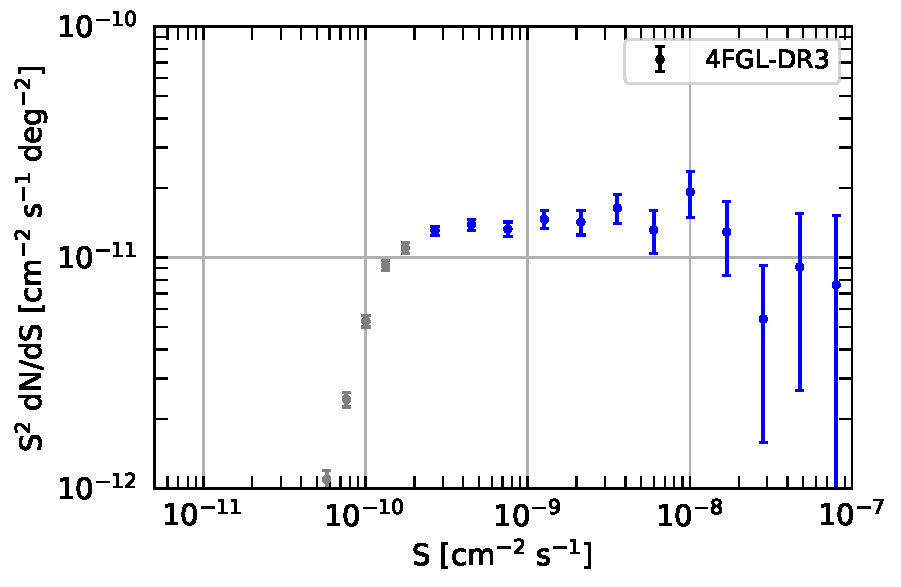
\includegraphics[width=0.49\textwidth]{img/data_selection/4FGL.pdf}
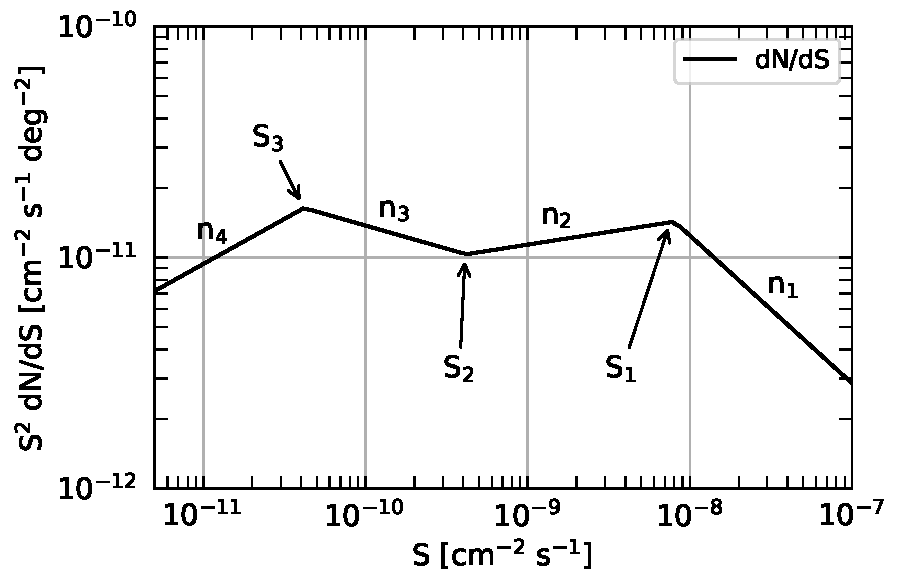
\includegraphics[width=0.49\textwidth]{img/data_selection/dNdS_annotato.pdf}
\caption{Left: The 1-10 GeV $\dnds$ for resolved \fermi sources, obtained from the 4FGL-DR3 \cite{2022ApJS..260...53A} catalog. Right: An example of $dN/dS$ with 3 breaks $S_j$ ($j=1,3$) and four slopes, where $n_i$ ($i=1,4$) is the inclination of the slope.}
\label{fig:dNdS-annotato}
\end{figure}


\begin{table}[t]
\centering
\begin{tabular}{lllcc}
\hline
 & Parameter & Prior & Range \\
\hline & $A_{S}$ & log-flat & {$[1,\, 15]$} \\
& $F_\textrm{iso}$ & log-flat & {$[0.5 \cdot 10^{-7},\, 7.0 \cdot 10^{-7}]$} \\
\hline &
$S_{1}$ & log-flat & {$[3 \cdot 10^{-9}, 5.0 \cdot 10^{-8}]$ } \\
& $S_{2}$ & log-flat & {$[5 \cdot 10^{-11}, 3.0 \cdot 10^{-9}]$} \\ 
& $S_{3}$ & log-flat & {$[5\cdot 10^{-12},5\cdot 10^{-11}]$} \\
& $n_{1}$ & flat & {$[2,\, 4]$} & \\
& $n_{2}$ & flat & {$[1.80,\, 2.15]$} & \\
& $n_{3}$ & flat & {$[1.5,\, 2.5]$} & \\
& $n_{4}$ & flat & {$[1.0,\, 3.0]$} & \\
\hline 
\end{tabular}
\caption{Ranges of the parameters and their sampling priors adopted in the map generation with $N_b = 3$ breaks. The normalization $A_S$ is in units of $10^7$ cm$^2$ s sr$^{-1}$. $F_\textrm{iso}$ is in units of cm$^{-2}$ s$^{-1}$ sr$^{-1}$. The breaks $S_{1}$ $S_{2}$ and $S_{3}$ are given in units of cm$^{-1}$s$^{-1}$. All other quantities are dimensionless.}
\label{tab:prior-dNdS}
\end{table}

Following \cite{Cuoco-1pdf}, the differential source-count distribution $\dnds$ is modeled as a multi-break power-law (MBPL). A MBPL with $N_b$ breaks located at fluxes $S_{j}$ ($j = 1, 2, ..., N_b$) is defined as:


\begin{equation}
\frac{d N}{d S} = A_S \times \left\{\begin{array}{lr}
\left(\frac{S}{S_{0}}\right)^{-n_{1}}, & \quad S>S_{1} \\ \\
\left(\frac{S_{1}}{S_{0}}\right)^{-n_{1}+n_{2}}\left(\frac{S}{S_{0}}\right)^{-n_{2}}, &\quad S_{2}<S \leqslant S_{1} \\ 
\vdots\\\vdots \\
\left(\frac{S_{1}}{S_{0}}\right)^{-n_{1}+n_{2}}\left(\frac{S_{2}}{S_{0}}\right)^{-n_{2}+n_{3}} \cdots\left(\frac{S}{S_{0}}\right)^{-n_{N_{b}+1}}, &\quad S \leqslant S_{N_{b}}
\end{array}\right.
\end{equation}

\begin{figure}[t]
\centering
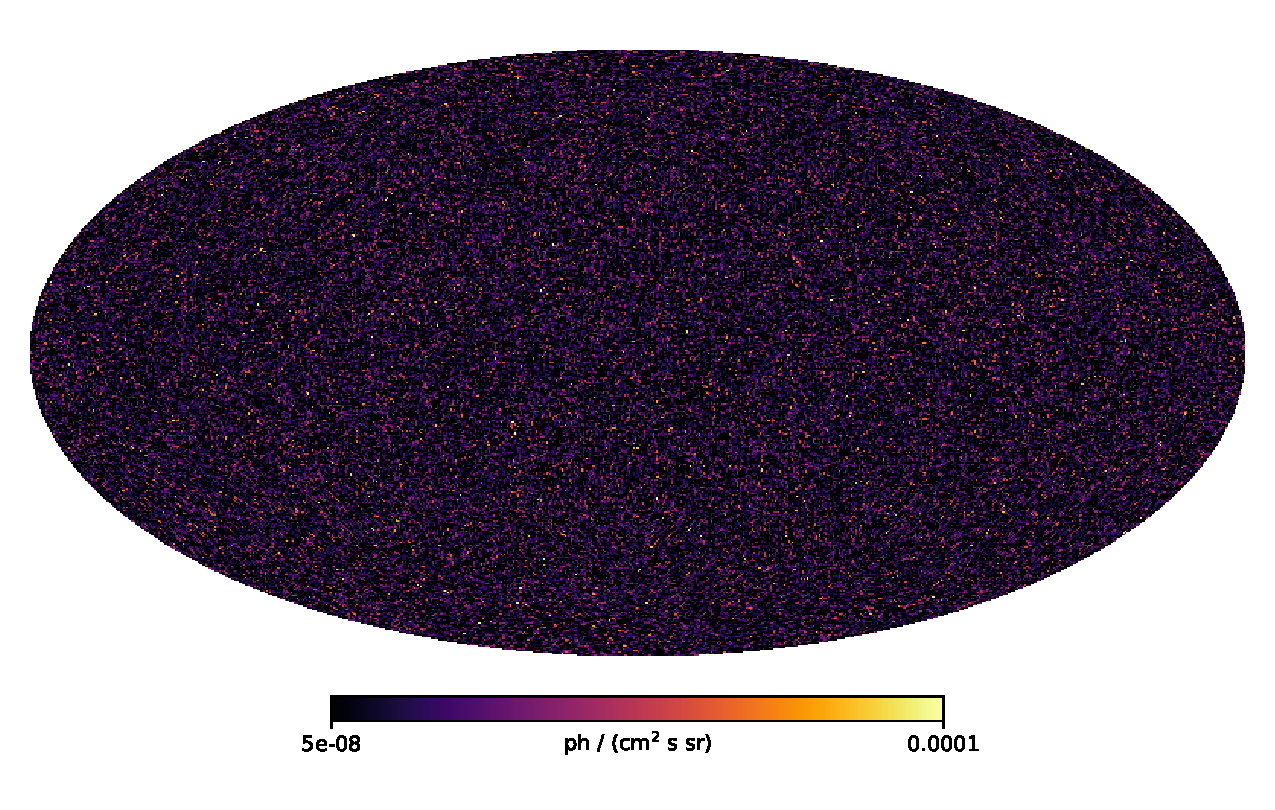
\includegraphics[scale=0.60]{img/data_selection/point_sources.pdf}
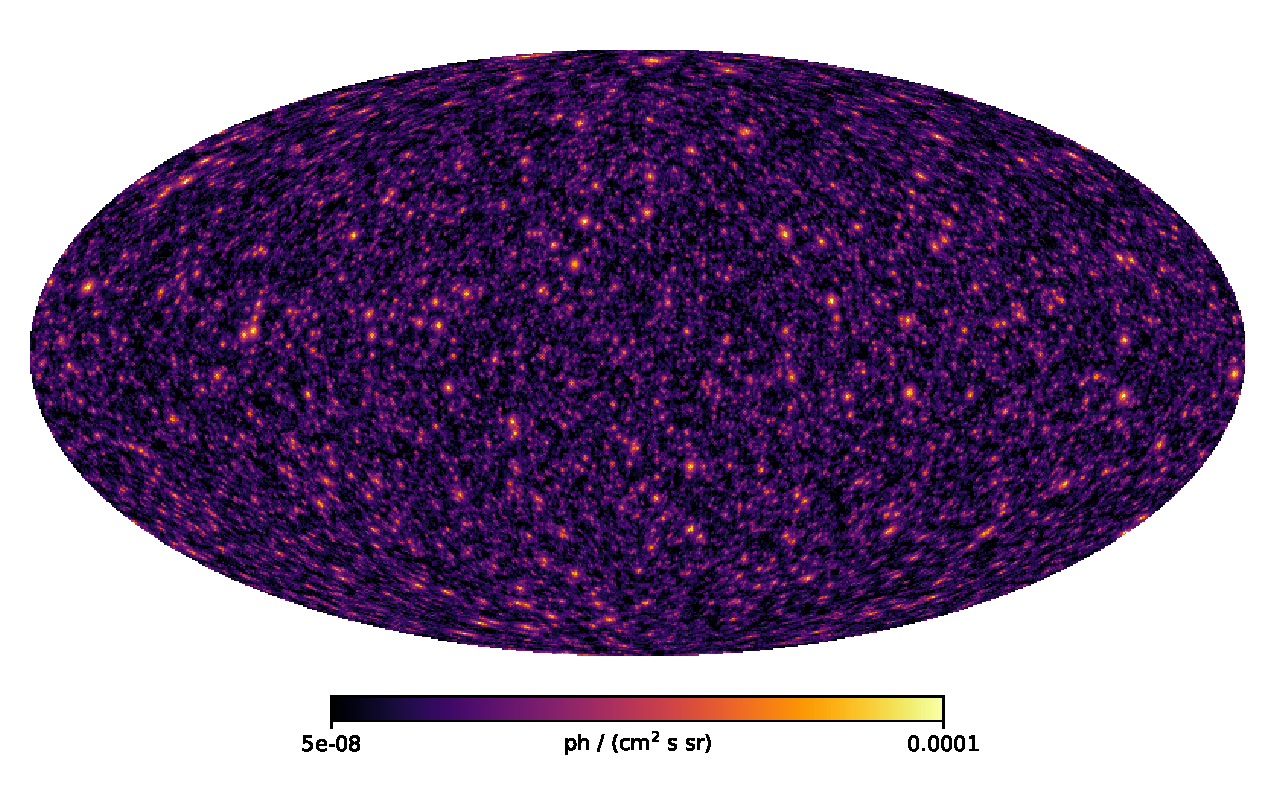
\includegraphics[scale=0.60]{img/data_selection/smoothed_PS.pdf}
\caption{Simulated flux map of point sources extracted from a specific source-count distribution, before (upper panel) and after (lower panel) the PSF is applied, in units of photons/(cm$^2$ s sr). The maps are shown at Healpix resolution $N_\textrm{side} = 128$ ($n=7$). 
}
\label{fig:point-sources}
\end{figure}


\noindent
where $S_0$ is a reference flux value which we choose to be $S_0 = 3 \cdot 10^{-8} \textrm{cm}^{-2} \textrm{s}^{-1}$,  and $n_j$ are the power-law indices. $S$ denotes the source flux in the energy interval $(1,10)$ GeV. The $dN/dS$ distribution is normalized with an overall factor $A_S$. 

For definiteness, in this work we adopt 3 breaks and 4 slopes. The ranges in which the parameters are varied to produce different source-count distributions is reported in Table \ref{tab:prior-dNdS}. The ranges have been chosen in order to intercept the expected features of the $\dnds$ and are broad enough to allow for a good variability in the modeling of the source counts, in order to expose the CNN to a wide set of options. In fact, the prior ranges of the three break positions are chosen relative to the \fermi threshold for resolving point sources, $S_\textrm{th} \sim 2 \cdot 10^{-10}$ cm$^{-2}$ s$^{-1}$, such that $S_1$, $S_2$, $S_3$ are respectively larger, across and below $S_\textrm{th}$. The flux interval over which we will try to reconstruct the $\dnds$ is set as $[5 \cdot 10^{-12}, 1 \cdot 10^{-7}]$ cm$^{-2}$ s$^{-1}$. The upper limit of this interval is set by the brightest sources in the catalog, while the lower limit is set at about 1.6 orders of magnitude below the \fermi threshold for resolving sources. Sources fainter than the lower limit of this interval are assumed to just contribute to the isotropic component.
{  This lower limit, indeed, is also close to the theoretical sensitivity given by the flux of a point source contributing exactly one photon, which we calculate as $F_\textrm{sens}= 1/{\cal E}_{av}=3.74 \cdot 10^{-12}$ cm$^{-2}$ s$^{-1}$  where ${\cal E}_{av}$ is the average exposure in the region $|b|>30^\circ$ where we perform the analysis.}





The prior ranges for the power-law slopes are anchored to the results from the 4FGL catalog in the resolved regime, and allow for progressively wider variability moving toward the unresolved regime. Since catalog data exhibit a source count compatible with $S^{-2}$, except for large fluxes, where the slope increases, we adopt priors for $n_1$ and $n_2$ around these behaviours. For $n_3$ and $n_4$, we progressively enlarge the prior ranges, in order to allow for more variability especially in the sub-threshold (unresolved) regime we are interested in. An example of a $\dnds$ generated from this procedure is shown in the right panel of Fig. \ref{fig:dNdS-annotato}, which also illustrates the notation.

The maps {$\cal S$} are generated according to the following procedure:
\begin{enumerate}
\item A $\dnds$ is selected by random sampling of its parameters in the intervals and with the priors defined in Table \ref{tab:prior-dNdS};

\item The number $N_i$ of sources in the $i$th flux bin is calculated as $N_i = 4\pi \, (S_{i, \rmfamily max} - S_{i, \rmfamily min}) \, \dnds|_i$ where $\dnds|_i$ is the value at the center of the $i$th bin. The flux bins are determined by subdividing the interval of interest {$[5 \cdot 10^{-12}, 1 \cdot 10^{-7}]$ } cm$^{-2}$ s$^{-1}$ in $10^3$ log-intervals per decade;

\item A Poisson extraction on $N_i$ determines the number of sources $N_{P,i}$ in each flux interval;

\item The sources are randomly positioned on the sphere by uniformly sampling $\cos\theta$ in $[-1,1]$ and $\varphi$ in $[0, 2\pi]$, $\theta$ and $\varphi$ being the spherical coordinates. The selected angular position is then converted into a pixel position in the Healpix pixeling scheme with the {\tt ang2pix} routine. An example of a point-source map is shown in the upper panel of Fig. \ref{fig:point-sources};

\item Finally, convolution with the \fermi PSF shown in Fig. \ref{fig:PSF} is applied to each point source. Since sources are assumed to be point-like, we simply replace each point source with an extended circular object with a radial profile equal to the PSF, and whose total flux is equal to the one of the original source. Since the image formation process is linear in the intensity, in case of overlapping sources (either because of their spatial position, or because of the PSF smearing) the resulting flux is additive. An example of flux map with the PSF applied is shown in the lower panel of Fig. \ref{fig:point-sources}.
\end{enumerate}

In order to avoid possible biases in the generated maps, due to the resolution of the angular binning, the maps generated with the procedure described above have been produced at a resolution higher than the one adopted for the analysis. We have therefore built our maps with $N_\textrm{side} = 128$. These maps have then been downgraded to $N_\textrm{side} = 64$ for the analysis.

\subsection{Galactic foreground and isotropic background}
\label{sec:galactic}

\begin{figure}[t]
\centering
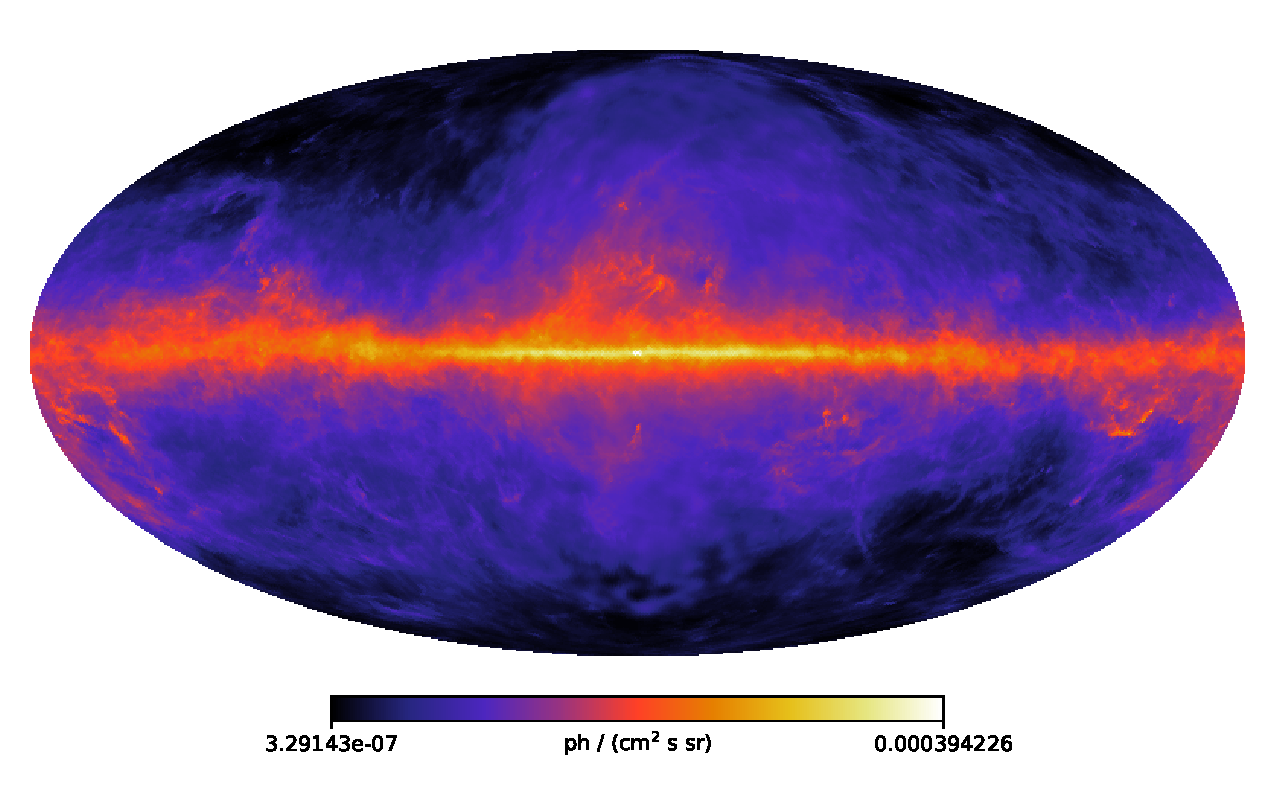
\includegraphics[scale=0.6]{img/data_selection/gf7.pdf}
\caption{$\tt {gll\_iem\_v07}$ galactic foreground model \cite{4FGL}, integrated in the $(1,10)$ GeV energy bin, in units of photons/(cm$^2$ s sr), at the Healpix resolution $N_\textrm{side} = 128$ ($n=7$).}
\label{fig:galactic-foreground}
\end{figure}

The galactic foreground is implemented through the adoption of the \fermi template model \verb|gll_iem_v07|\footnote{\url{https://fermi.gsfc.nasa.gov/ssc/data/access/lat/BackgroundModels.html}}. 
The map of the integrated flux in the $(1, 10)$ GeV energy range is shown in Fig. \ref{fig:galactic-foreground}. To check consistency and stability of our results, we will also adopt a different version of the galactic template, namely model \verb|gll_iem_v05|\footnotemark[\value{footnote}]. The extragalactic isotropic background instead is modeled as a constant flux $\fiso$, which captures all the unresolved emission which is too faint to be associated to the emission modeled through the $\dnds$ (i.e., which refers to fluxes $S<5 \cdot 10^{-12}$ cm$^{-2}$ s$^{-1}$, below our region of interest).

As shown in Fig. \ref{fig:galactic-foreground}, the galactic foreground dominates at low latitudes, although it extends to high latitudes with a smaller flux. For these reasons, low latitudes are unsuitable for the study of the extra-galactic background. Our baseline analysis will therefore apply a mask to the maps to cover the dominant part of the galactic emission, for which we adopt a latitude cut $|b|<30^\circ$. In order to check the stability of the results against the foreground treatment, in Section \ref{sec:results} we will show the results obtained with two additional latitude cuts: $|b|<40^\circ$ and $|b|<50^\circ$.

Given the various approximations we use, instead of using the nominal normalization of the galactic foreground models, we prefer to use a data-driven approach and normalize 
the galactic templates \verb|gll_iem_v07| and \verb|gll_iem_v05| directly to the observed \fermi map. This is realized by performing a maximum-likelihood Poisson fit, using as likelihood:
%
\begin{equation}
\mathcal{L}=\prod_{a=1}^{N_\textrm{pix}} \frac{\lambda_{a}^{k_{a}} e^{-\lambda_{a}}}{k_{a} !}
\end{equation}
%
where $k_a$ is the number of photons in pixel $a$ of the \fermi count map and $\lambda_a$ the corresponding quantity from the model count-map, given by $\lambda_a = (A_\textrm{gal}\ {\cal G}_a + F'_\textrm{iso}) \cdot {\cal E}_a \cdot \frac{4\pi}{N_\textrm{pix}} $, where $A_\textrm{gal}$ and $F'_\textrm{iso}$ are the two fit parameters. In performing the fit we mask the sky with the low-latitude cut and with a $2^\circ$ circular mask around each of the sources in the 4FGL catalog. 
We added a prime on the $F'_\textrm{iso}$ derived from the maximum-likelihood fit above to explicitly distinguish it from the $F_\textrm{iso}$ introduced earlier.
Confronting with Eq. (\ref{eq:map}), the $F'_\textrm{iso}$ term denotes the sum of the purely isotropic contribution $F_\textrm{iso}$  and the contribution of sources, ${\cal S}$ term, below the 4FGL detection threshold.


\begin{table}[t]
\centering
\begin{tabular}{|l|c|c|c|}
\hline
Foreground template & Latitude cut & $A_\textrm{gal}$ & $F'_\textrm{iso}$ \\
\hline
\verb|gll_iem_v07| & $|b|<30^\circ$ & $0.888 \pm 0.005$ & $(4.91  \pm 0.04 ) \cdot 10^{-7}$ \\
\verb|gll_iem_v07| & $|b|<40^\circ$ & $0.874 \pm 0.008$ & $(4.90  \pm 0.06 ) \cdot 10^{-7}$ \\
\verb|gll_iem_v07| & $|b|<50^\circ$ & $0.838 \pm 0.013$ & $(5.05  \pm 0.08 ) \cdot 10^{-7}$ \\
\hline
\verb|gll_iem_v05| & $|b|<30^\circ$ & $1.030 \pm 0.006$ & $(2.57  \pm 0.06 ) \cdot 10^{-7}$ \\
\hline 
\end{tabular}
\caption{Values of the $A_\textrm{gal}$ and $F'_\textrm{iso}$ parameters obtained from a fit to the \fermi map, for different galactic foreground template models and latitude cuts. $F'_\textrm{iso}$ is in units of cm$^{-2}$ s$^{-1}$ sr$^{-1}$.}
\label{tab:fore-parameters}
\end{table}

The results of the fit are shown in Table \ref{tab:fore-parameters}, for three latitude cuts for the \verb|gll_iem_v07| template and for $|b|<30^\circ$ for the alternative \verb|gll_iem_v05| model. We see that both the normalisation parameter $A_\textrm{gal}$ and $F'_\textrm{iso}$ are consistent among themselves for a fixed galactic foreground model, implying consistency with respect to the latitude cut. The model \verb|gll_iem_v05| instead requires a larger normalization, with an ensuing reduced value for $F'_\textrm{iso}$ by a factor of 2.
This reflects a certain amount of degeneracy which is present at high galactic latitude between the foreground emission and the isotropic emission, allowed by the uncertainties in the foreground model.
The normalization of the \verb|v07| model different from 1 is related to the fact that we do not include energy dispersion. The \verb|v05| model, instead, has been created originally without including the effect of energy dispersion\footnote{\url{https://fermi.gsfc.nasa.gov/ssc/data/access/lat/BackgroundModels.html}}, and indeed we obtain a normalization compatible with 1.


Throughout the rest of the analysis we will fix the normalization parameter $A_\textrm{gal}$ to the value determined from the above fit. The values of $F'_\textrm{iso}$ are, instead, used to define the range of the prior for $F_\textrm{iso}$ in Table \ref{tab:prior-dNdS} and \textsl{a posteriori} to check consistency of the results.
%
One illustration of a flux map obtained as the sum of all components is shown in Fig. \ref{fig:map_with_gf}.
Instead of fixing $A_\textrm{gal}$, in principle, we could also leave it as a free parameter and instruct the network to predict its value. We found, however, that the above procedure constrains $A_\textrm{gal}$ very precisely and it is thus preferable. Furthermore, we also found that fixing $A_\textrm{gal}$ provides a better stability of the neural network.  

{  Nonetheless, to better asses the impact of fixing the $A_\textrm{gal}$ value, we also performed a further test using different values in the range $(0.78, 1.0)$ (i.e., a range centered on our fiducial value $0.888 \pm 0.005$, thus encompassing many standard deviations away from its central value.)
We found that the $\dnds$ reconstructed by the CNN is largely unaffected by the employed value of $A_\textrm{gal}$, while 
the specific $A_\textrm{gal}$ choice mostly affect $F_\textrm{iso}$,
as expected because of the  high galactic latitude degeneracy between the foreground emission and the isotropic emission. 
Example plots are shown in the Appendix \ref{sec:agal-var}.}





\subsection{Count maps}

With a flux map ${\cal M}$ available, we can now produce a synthetic photon-count map ${\cal N}$ as described in Eq. \ref{eq:count}. 
One example is shown in Fig. \ref{fig:map-total-counts}. 
In order to generate maps compatible with a counting experiment like \fermi, we then add Poisson noise to the map performing a Poisson realization of the number of photons in each pixel of the map ${\cal N}$, and we dub this final map as ${\cal N}_{\cal P}$ count map. One example is shown in Fig. \ref{fig:map-effective}, which also shows the same map with the latitude cut applied: these are the type of maps that we use to train and validate the neural network. We have generated in total 1 million maps, 90\% of which have been used for training and 10\% for validation. The maps have been stored as a \verb|TFRecord| dataset\footnote{\texttt{https://www.tensorflow.org/tutorials/load\_data/tfrecord}} for use with Tensorflow \cite{tensorflow2015-whitepaper}. The maps have been generated in Healpix format with $N_\textrm{side} = 128$ resolution (order $n=7$) and then downsampled to $N_\textrm{side} = 64$ (order $n=6$) for the training and validation (this resolution corresponds to 49152 pixels). 

The training of the CNN and the subsequent analysis of the \fermi data can be performed equivalently with maps in units of photon-count or in units of flux. Nonetheless, we will work with maps in units of flux, which are easily obtained from the ${\cal N}_{\cal P}$ count maps by using the exposure map and by inverting Eq. (\ref{eq:count}).  The reason to convert the ${\cal N}_{\cal P}$ count maps in units of flux is motivated by the fact that 
count maps contain a spurious large-scale angular dependence
introduced by the exposure map (see Fig. \ref{fig:exposure}) which
might confuse the CNN, while this potential issue is avoided
using flux maps.
Finally, to further ease the learning process of the CNN
we also apply a foreground subtraction procedure,
i.e., to the above flux maps we subtract the original
galactic template flux map.
In this way the CNN can focus on learning the $\dnds$, seeing the exposure and galactic foregrounds only as sources of noise, instead of trying to learn their detailed structure. These foreground-subtracted flux maps are the maps we use to train the CNN. 

\begin{figure}[t]
\centering
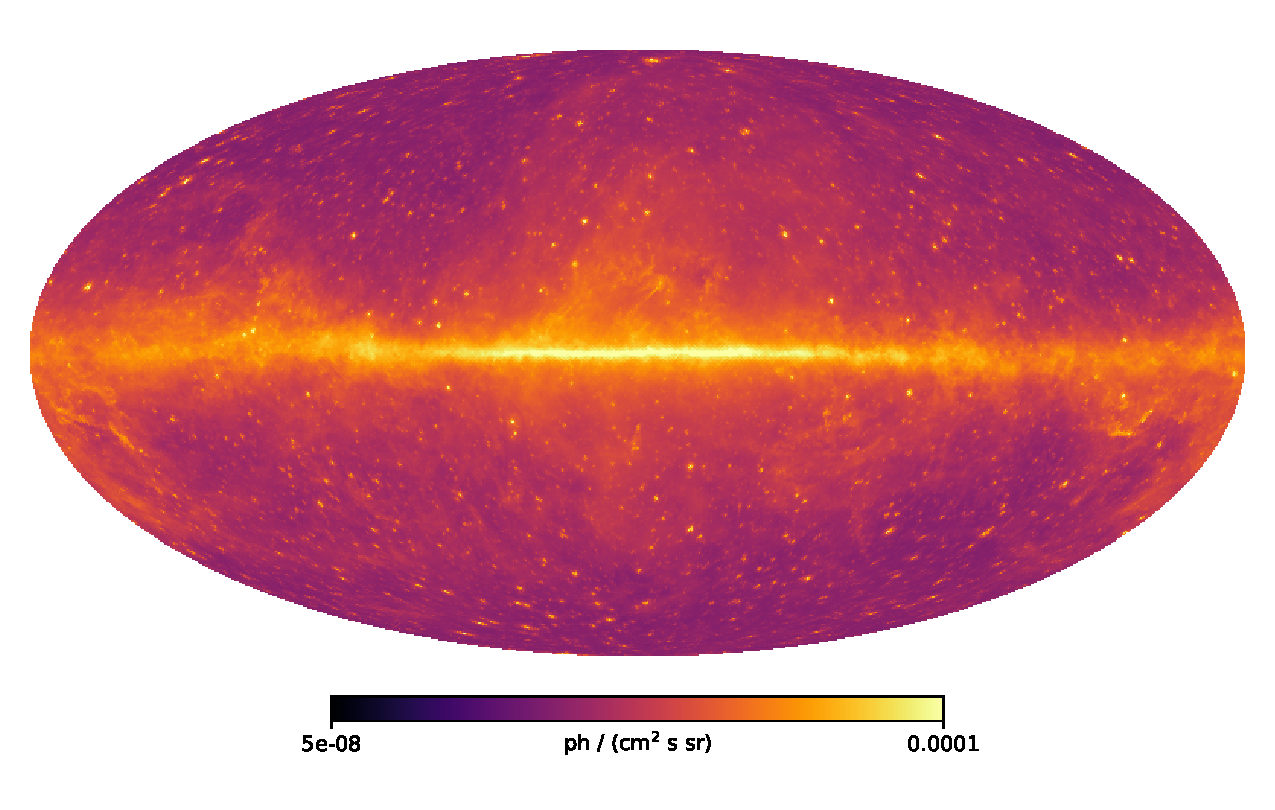
\includegraphics[scale=0.6]{img/data_selection/point_sources_fg.pdf}
\caption{The same as in Fig. \ref{fig:point-sources}, with the galactic foreground model normalized with $A_\textrm{gal} = 0.886$ and an isotropic background component $F_\textrm{iso} = 4 \cdot 10^{-7}$ cm$^{-2}$ s$^{-1}$ sr$^{-1}$. Units are photons/(cm$^2$ s sr).}
\label{fig:map_with_gf}
\end{figure}

\begin{figure}[h]
\centering
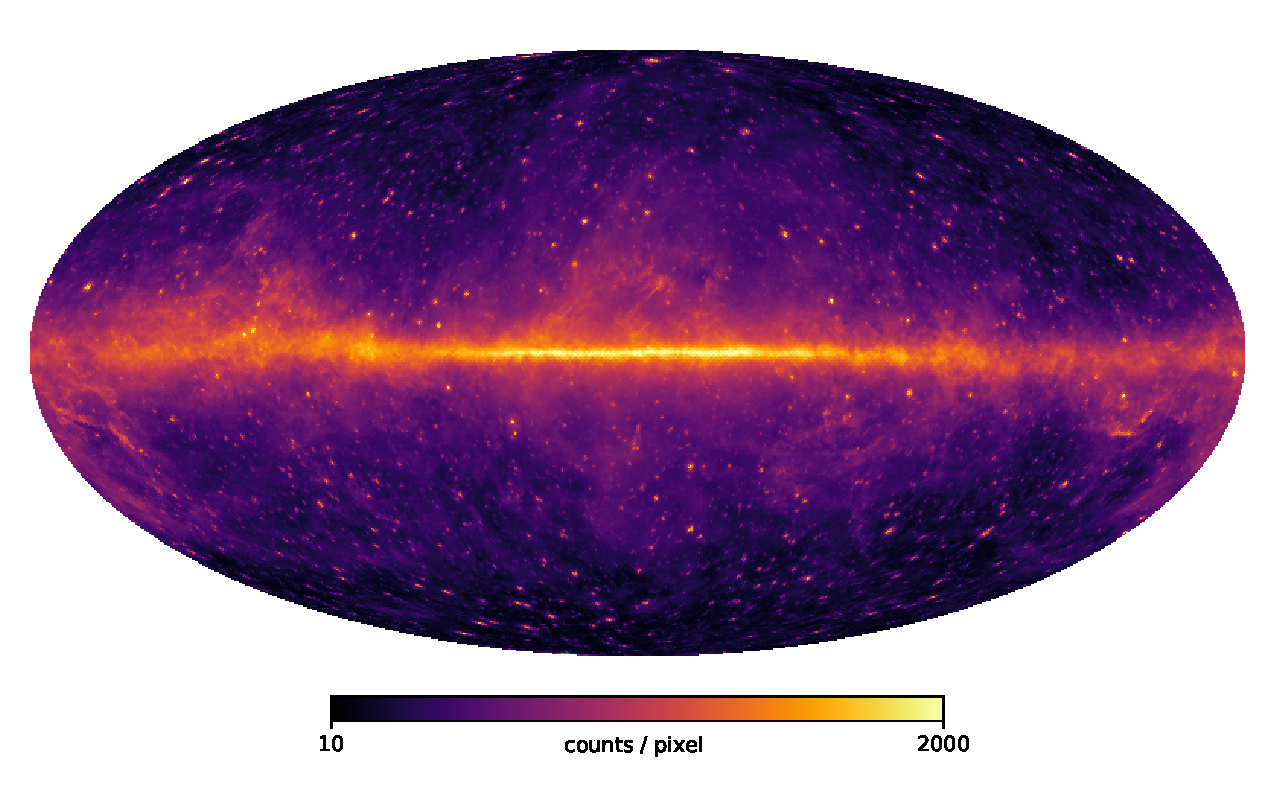
\includegraphics[scale=0.6]{img/data_selection/counts_map.pdf}
\caption{Simulated count map in units of counts per pixel,  at the Healpix resolution $N_\textrm{side} = 128$ ($n=7$). }
\label{fig:map-total-counts}
\end{figure}

\begin{figure}[h]
\centering
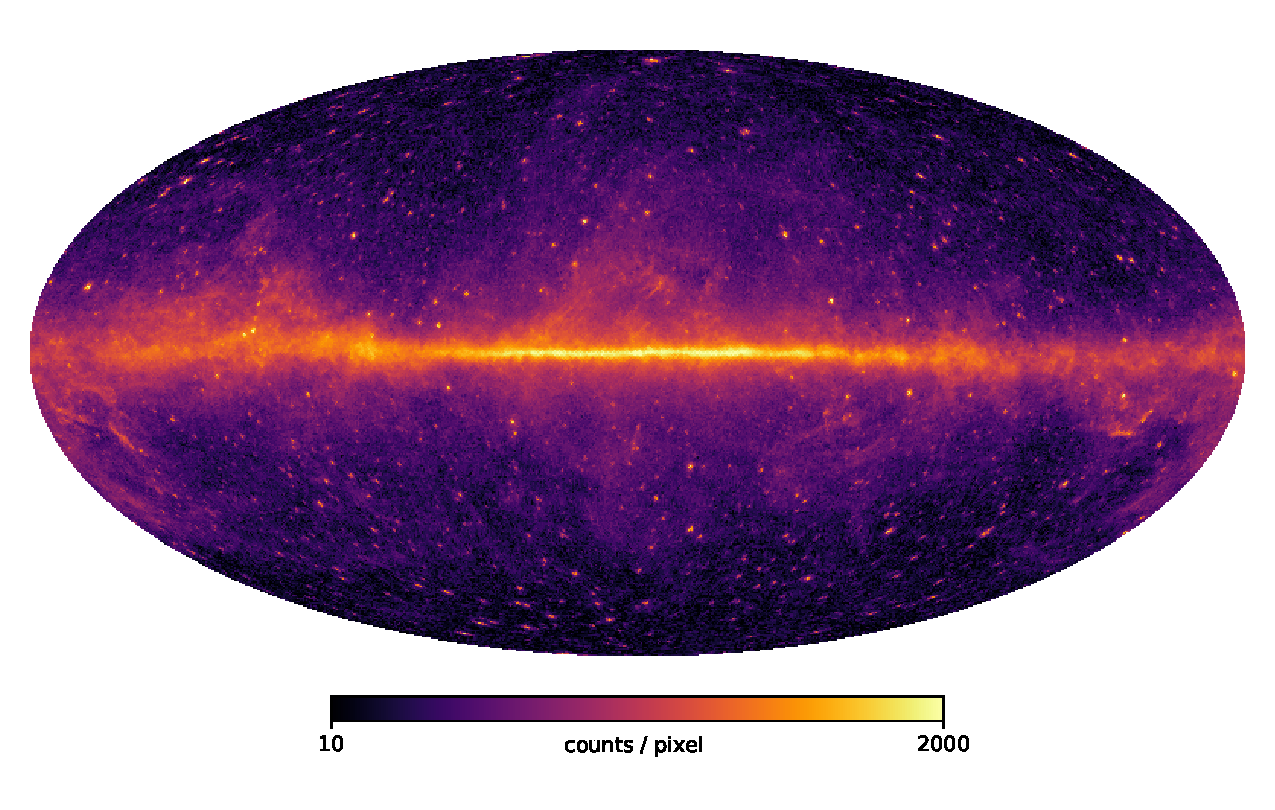
\includegraphics[scale=0.6]{img/data_selection/counts_map_effective.pdf}
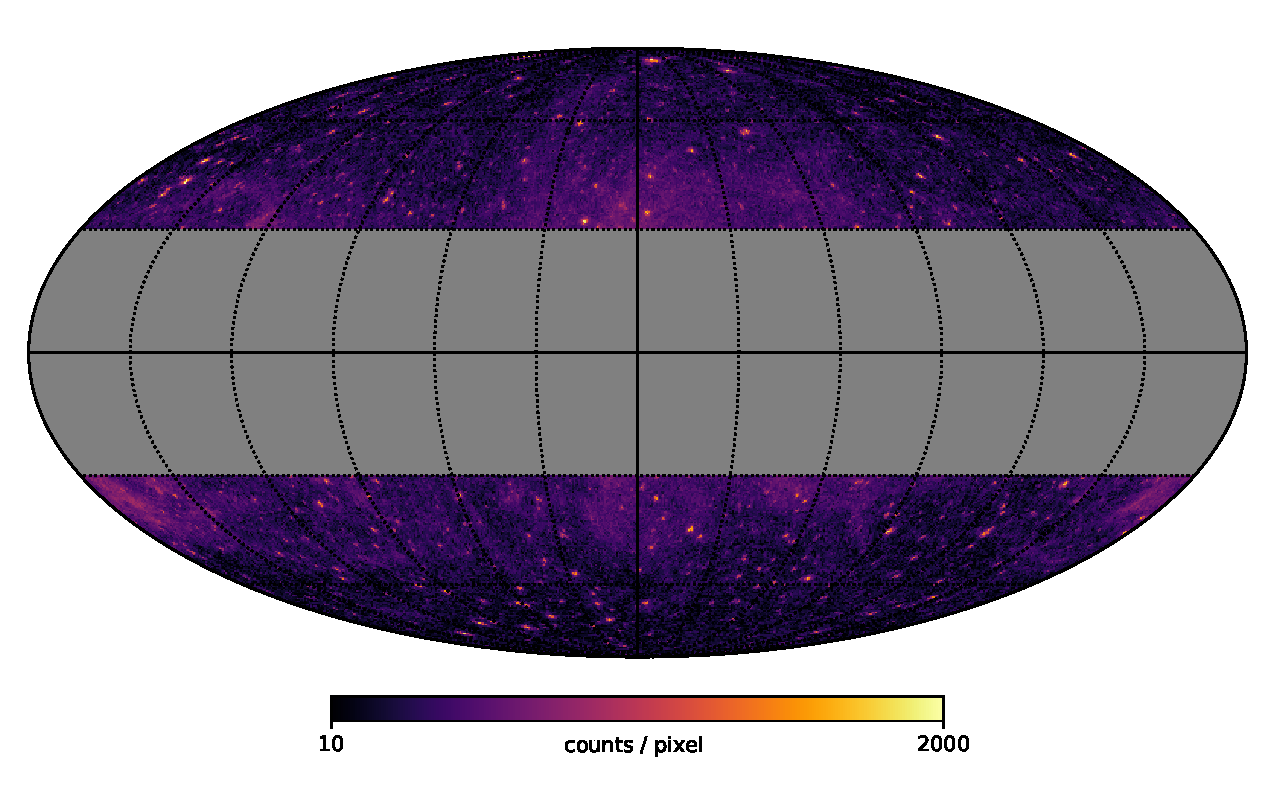
\includegraphics[scale=0.6]{img/data_selection/counts_map_effective_masked.pdf}
\caption{Simulated map in units of counts per pixel after  adding Poisson noise from the synthetic model map of Fig. \ref{fig:map-total-counts}, at the same Healpix resolution $N_\textrm{side} = 128$ ($n=7$). The lower panel shows the map with a $|b| < 30^\circ$ latitude cut.}
\label{fig:map-effective}
\end{figure}


%---------------------------------

